\documentclass[
	% -- opções da classe memoir --
	12pt,				% tamanho da fonte
	openright,			% capítulos começam em pág ímpar (insere página vazia caso preciso)
	oneside,			% para impressão em recto e verso. Oposto a oneside
	a4paper,			% tamanho do papel. 
	% -- opções da classe abntex2 --
	chapter=TITLE,		% títulos de capítulos convertidos em letras maiúsculas
	%section=TITLE,		% títulos de seções convertidos em letras maiúsculas
	%subsection=TITLE,	% títulos de subseções convertidos em letras maiúsculas
	%subsubsection=TITLE,% títulos de subsubseções convertidos em letras maiúsculas
	% -- opções do pacote babel --
	english,			% idioma adicional para hifenização
	french,				% idioma adicional para hifenização
	spanish,			% idioma adicional para hifenização
	brazil,				% o último idioma é o principal do documento
	]{abntex2}

% ---
% Pacotes fundamentais 
% ---
\usepackage{unijui}
\usepackage{lmodern}			% Usa a fonte Latin Modern			
\usepackage[T1]{fontenc}		% Selecao de codigos de fonte.
\usepackage[utf8]{inputenc}		% Codificacao do documento (conversão automática dos acentos)
\usepackage{lastpage}			% Usado pela Ficha catalográfica
\usepackage{indentfirst}		% Indenta o primeiro parágrafo de cada seção.
\usepackage{color}				% Controle das cores
\usepackage{graphicx}			% Inclusão de gráficos
\usepackage{microtype} 			% para melhorias de justificação
% ---

% ---
% Pacotes de citações
% ---
\usepackage[brazilian]{}

\usepackage{placeins}
\usepackage{multirow}
\usepackage[table]{xcolor}
\usepackage[pt-BR]{datetime2}
\newcommand\speedup{\textit{speed-up~}}
\newcommand{\charm}{\textsc{Charm++}\xspace}
\newcommand{\newlb}{\textsc{SmartLB }\xspace}
\newcommand{\hybridlb}{\textsc{HybridLB}\xspace}
\newcommand{\greedylb}{\textsc{GreedyLB}\xspace}
\newcommand{\refinelb}{\textsc{RefineLB}\xspace}
\newcommand{\rand}{\textsc{RandCentLB}\xspace}
\newcommand{\grapelb}{\textsc{GrapeVineLB}\xspace}
\newcommand{\grapepluslb}{\textsc{GrapePlusLB}\xspace}

\DTMlangsetup{showdayofmonth=false}

% ---
% Informações de dados para capa, folha de rosto e folha de aprovação
% ---
\titulo{SmartLB: Proposta de Balanceamento de Carga para Redução de tempo de execução em Ambientes Multiprogramados}
\autor{Vinicius Ribas Samuel dos Santos}
\local{Ijuí/RS}
\data{2017}
\instituicao{%
   Universidade Regional do Noroeste do Estado do Rio Grande do Sul - UNIJUI}
\orientador{Professor DSc. Edson Luiz Padoin}
\tipotrabalho{Trabalho de Conclusão de Curso}
% O preambulo deve conter o tipo do trabalho, o objetivo, 
% o nome da instituição e a área de concentração 
\preambulo{Trabalho de Conclusão de Curso apresentado ao Colegiado de Coordenação do Curso de Ciência da Computação da Universidade Regional do Noroeste do Estado do Rio Grande do Sul (UNIJUÍ), como requisito parcial para obtenção do Título de Bacharel em Ciência da Computação.}


% ---
% Configurações de aparência do PDF final


% informações do PDF
\makeatletter
\hypersetup{
     	%pagebackref=true,
		pdftitle={\@title}, 
		pdfauthor={\@author},
    	pdfsubject={\imprimirpreambulo},
	    pdfcreator={LaTeX with abnTeX2},
		pdfkeywords={tcc}{computação}{ciência}, 
		colorlinks=true,       		% false: boxed links; true: colored links
    	linkcolor=black,          	% color of internal links
    	citecolor=black,        		% color of links to bibliography
    	filecolor=black,      		% color of file links
		urlcolor=black,
		bookmarksdepth=4
}
\makeatother
% --- 

% --- 
% Espaçamentos entre linhas e parágrafos 
% --- 

% O tamanho do parágrafo é dado por:
\setlength{\parindent}{1.3cm}

% Controle do espaçamento entre um parágrafo e outro:
\setlength{\parskip}{0.2cm}

% ---
% compila o indice
% ---
\makeindex
% ---

% ----
% Início do documento
% ----
\begin{document}

% Seleciona o idioma do documento (conforme pacotes do babel)
%\selectlanguage{english}
\selectlanguage{brazil}

% Retira espaço extra obsoleto entre as frases.
\frenchspacing 

% ---
% Capa
% ---

\imprimircapa
% ---

% ---
% Folha de rosto
% (o * indica que haverá a ficha bibliográfica)
% ---

\imprimirfolhaderosto*

% ---

% ---
% Inserir a ficha bibliografica
% ---

% Isto é um exemplo de Ficha Catalográfica, ou ``Dados internacionais de
% catalogação-na-publicação''. Você pode utilizar este modelo como referência. 
% Porém, provavelmente a biblioteca da sua universidade lhe fornecerá um PDF
% com a ficha catalográfica definitiva após a defesa do trabalho. Quando estiver
% com o documento, salve-o como PDF no diretório do seu projeto e substitua todo
% o conteúdo de implementação deste arquivo pelo comando abaixo:
%
% \begin{fichacatalografica}
%     \includepdf{fig_ficha_catalografica.pdf}
% \end{fichacatalografica}

% ---
% Inserir folha de aprovação
% ---

% Modelo de folha de aprovação utilizado na UNIJUI, elemento obrigatório da NBR
% 14724/2011 (seção 4.2.1.3). Você pode utilizar este modelo até a aprovação
% do trabalho. Após isso, substitua todo o conteúdo deste arquivo por uma
% imagem da página assinada pela banca com o comando abaixo:
%
% \includepdf{folhadeaprovacao_final.pdf}
%


\newcommand{\imprimirfolhaaprovacao}{%
	\begin{folhadeaprovacao}		
	\begin{center}
		\ABNTEXchapterfont\mdseries\large\MakeUppercase\imprimirinstituicao
		
		\vspace*{5mm}
		
		A Comissão Examinadora, abaixo assinada, aprova o \imprimirtipotrabalho:
		
		\vspace*{5mm}
		
		\ABNTEXchapterfont\large\bfseries\MakeUppercase\imprimirtitulo\mdseries
		
		\vspace*{5mm}
		
		Elaborado por
		
		\vspace*{5mm}
		
		\ABNTEXchapterfont\mdseries\large\MakeUppercase\imprimirautor
		
		\vspace*{5mm}
		
		Como requisito parcial para obtenção do título de Bacharel em Ciência da Computação
		
		\vspace*{\fill}
		
		Comissão Examinadora
		
		\assinatura{\textbf{\imprimirorientador} \\ Orientador} 
		\assinatura{\textbf{Professor} \\ Convidado 1}
		\assinatura{\textbf{Professor} \\ Convidado 2}
		%\assinatura{\textbf{Professor} \\ Convidado 3}
	
		\vspace*{\fill}
		{\large\imprimirlocal}
		
		\par
		
		%A data de aprovação e as assinaturas dos membros componentes da banca examinadora devem ser colocadas após a aprovação do trabalho.		
		{\large 17 de Junho de 2017}
	\end{center}	
	\end{folhadeaprovacao}
}

% \imprimirfolhaaprovacao

% ---

% ---
% Dedicatória (OPCIONAL)
% ---
\begin{dedicatoria}
    \vspace*{\fill}
	\begin{flushright}
		\textit{Lorem ipsum dolor sit amet, consetetur sadipscing elitr, sed diam nonumy eirmod tempor invidunt ut labore et dolore magna aliquyam erat, sed diam voluptua. At vero eos et accusam et justo duo dolores et ea rebum. Stet clita kasd gubergren, no sea takimata sanctus est Lorem ipsum dolor sit amet. Lorem ipsum dolor sit amet, consetetur sadipscing elitr, sed diam nonumy eirmod tempor invidunt ut labore et dolore magna aliquyam erat, sed diam voluptua. At vero eos et accusam et justo duo dolores et ea rebum. Stet clita kasd gubergren, no sea takimata sanctus est Lorem ipsum dolor sit amet. Lorem ipsum dolor sit amet, consetetur sadipscing elitr, sed diam nonumy eirmod tempor invidunt ut labore et dolore magna aliquyam erat, sed diam voluptua. At vero eos et accusam et justo duo dolores et ea rebum. Stet clita kasd gubergren, no sea takimata sanctus est Lorem ipsum dolor sit amet.}
	\end{flushright}
\end{dedicatoria}
% ---
% Agradecimentos
% ---
\begin{agradecimentos}

Lorem ipsum dolor sit amet, consetetur sadipscing elitr, sed diam nonumy eirmod tempor invidunt ut labore et dolore magna aliquyam erat, sed diam voluptua. At vero eos et accusam et justo duo dolores et ea rebum. Stet clita kasd gubergren, no sea takimata sanctus est Lorem ipsum dolor sit amet. Lorem ipsum dolor sit amet, consetetur sadipscing elitr, sed diam nonumy eirmod tempor invidunt ut labore et dolore magna aliquyam erat, sed diam voluptua. At vero eos et accusam et justo duo dolores et ea rebum. Stet clita kasd gubergren, no sea takimata sanctus est Lorem ipsum dolor sit amet. Lorem ipsum dolor sit amet, consetetur sadipscing elitr, sed diam nonumy eirmod tempor invidunt ut labore et dolore magna aliquyam erat, sed diam voluptua. At vero eos et accusam et justo duo dolores et ea rebum. Stet clita kasd gubergren, no sea takimata sanctus est Lorem ipsum dolor sit amet.

Duis autem vel eum iriure dolor in hendrerit in vulputate velit esse molestie consequat, vel illum dolore eu feugiat nulla facilisis at vero eros et accumsan et iusto odio dignissim qui blandit praesent luptatum zzril delenit augue duis dolore te feugait nulla facilisi. Lorem ipsum dolor sit amet, consectetuer adipiscing elit, sed diam nonummy nibh euismod tincidunt ut laoreet dolore magna aliquam erat volutpat.

Ut wisi enim ad minim veniam, quis nostrud exerci tation ullamcorper suscipit lobortis nisl ut aliquip ex ea commodo consequat. Duis autem vel eum iriure dolor in hendrerit in vulputate velit esse molestie consequat, vel illum dolore eu feugiat nulla facilisis at vero eros et accumsan et iusto odio dignissim qui blandit praesent luptatum zzril delenit augue duis dolore te feugait nulla facilisi.

\end{agradecimentos}
% ---

% ---
% Epígrafe
% ---
\begin{epigrafe}
	\vspace*{\fill}
	\begin{flushright}
		\textit{"A imaginação é mais importante que o conhecimento. O conheicmento é limitado. A imaginação circunda o mundo."}   

        \textit{(Albert Einstein)}
	\end{flushright}
\end{epigrafe}
% ---

% ---
% RESUMO
% ---
\setlength{\absparsep}{18pt} % ajusta o espaçamento dos parágrafos do resumo
\begin{resumo}
	% tema
Este artigo apresenta uma proposta de balanceamento de carga para a redução do tempo de execução de aplicações paralelas executadas em ambientes multiprocessados.
% obj
O algoritmo do balanceador coleta informações do sistema e da aplicação em tempo real e as utiliza na tomada de decisões de balanceamento de carga dinamicamente, visando reduzir o número de migrações de tarefas enquanto reduzindo o tempo total de execução.  
% met
Para implementação foi utilizado o modelo de programação paralela \charm. 
% res
Os resultados preliminares apresentaram reduções de $3$ à $137$ vezes na quantidade de migrações de tarefas e reduções de $3,5$\% à $19,8$\% no tempo total de execução.	
\begin{comment}
Este trabalho trata de um tema bastante discutido atualmente, a computação paralela e heterogênea. Visa realizar a comparação de desempenho e eficiência energética de componentes que se enquadram nesta categoria. Para isso, serão comparados um coprocessador Intel Xeon Phi e uma GPGPU NVIDIA. Antes de compará-los, foi necessário um estudo das arquiteturas das GPUs da NVIDIA e do coprocessador Intel Xeon Phi (Intel MIC), bem como de algumas APIs e plataformas que possibilitam a implementação nestes componentes. A comparação foi realizada utilizando um \textit{benchmark}, que igualmente foi estudado. Como resultado, percebeu-se o quão eficientes ambos os componentes podem ser, no caso do Xeon Phi, que no \textit{benchmark} \textit{MaxFlops}, alcançou 5,06 TFlops para valores de precisão simples com uma eficiência energética de 17,27 GFlops/W e, na GPGPU NVIDIA, que no \textit{benchmark} GEMM, atingiu 3,03 TFlops para valores de precisão simples e uma eficiência energética de 13,18 GFlops/W. 


- O resumo deve responder 4 perguntas:

	a) qual o tema do trabalho; 

	b) qual o objetivo; 

	c) qual a metodologia empregada; e 

	d) qual o resultado/conclusão do trabalho.




\textbf{Palavras-chave}: Computação Paralela, Computação Heterogênea, Computação de Alto Desempenho, CUDA, OpenCL, OpenMP, SHOC \textit{Benchmark Suite}.
\end{comment}
\end{resumo}
% ---
% ABSTRACT
% ---
% resumo em inglês
\begin{resumo}[Abstract]
 \begin{otherlanguage*}{english}
This paper presents a load balancer proposal to reduce the execution time of  parallel applications when they run on multiprocessors environments. The load balancer algorithm collects system and application information in real time and uses them to make load balancing decisions dynamically, aiming to reduce the rate of migration and to decrease the execution time. \charm was used for implementation due to its compatibility with the desired environments. The results show that our load balancer improves performance by reducing task migration from $3$ up to $137$ times and reductions from  $3.5$\% to $19.8$\%  on total execution time.
\begin{comment}

\textbf{}
This paper deals with a topic that is much discussed at present, parallel and heterogeneous computing. It aims at comparing the performance and energy efficiency of components that fall into this category. For this, an Intel Xeon Phi coprocessor and an NVIDIA GPGPU will be compared. Before comparing them, a study of the NVIDIA GPU architectures and the Intel Xeon Phi coprocessor (Intel MIC) was needed, as well as some APIs and platforms that enable the implementation of these components. The comparison was performed using a benchmark, which was also studied. As a result, it was realized how efficient both components may be, in the case of Xeon Phi, that in the benchmark MaxFlops reached 5.06 TFlops for single precision values with an energy efficiency of 17,27 GFlops/W, and in NVIDIA GPGPU, which in the GEMM benchmark, reached 3.03 TFlops for single precision values and an energy efficiency of 13.18 GFlops/W. 

     \textbf {Keywords}: Parallel Computing, Heterogeneous Computing, High Performance Computing, CUDA, OpenCL, OpenMP, SHOC Benchmark Suite.
\end{comment}
 \end{otherlanguage*}
\end{resumo}
% ---
% inserir lista de ilustrações
% ---
\pdfbookmark[0]{\listfigurename}{lof}
\listoffigures*
\cleardoublepage
% ---
% inserir lista de tabelas
% ---
\pdfbookmark[0]{\listtablename}{lot}
\listoftables*
\cleardoublepage
% ---
% inserir lista de abreviaturas e siglas (OPCIONAL)
% ---
\begin{siglas}
  \item [BC] Balanceador de Carga
  \item [E/S] Entrada e Saída
  \item [FIFO] First In First Out
  \item [HPC] High Performance Computing
  \item [LIFO] Last In First Out
  \item [OOPP] Object Orientation Parallel Programming
  \item [PE] Processing Elemnents
  \item [RTS] Runtime System
\end{siglas}
% ---
% inserir lista de símbolos
% O caderno da UNIJUI não faz menção a símbolos. Se quiser usar é só descomentar.
% ---
% \begin{simbolos}
%   \item[$ \Gamma $] Letra grega Gama
%   \item[$ \Lambda $] Lambda
%   \item[$ \zeta $] Letra grega minúscula zeta
%   \item[$ \in $] Pertence
% \end{simbolos}
% ---
% ---
% inserir o sumario
% ---
\pdfbookmark[0]{\contentsname}{toc}
\tableofcontents*
\cleardoublepage
% ---
% ----------------------------------------------------------
% TEXTO
% ----------------------------------------------------------
\textual
\pagestyle{simple} 

\chapter{Introdução  \label{cap:introducao}}

A necessidade de alto desempenho, proveniente de um cresimento da produção de software deu abertura para o desenvolvimento dos sistemas computacionais, surgidos para suprir essa demanda \cite{artigoSalao2017}.

A medida que novas simulações computacionais são desenvolvidas, aumenta a demanda por processamento dos sistemas de HPC. Um dos componentes de hardware que apresentou uma enorme evolução foi o processador, que passou a proporcionar a execução simultanea de aplicações. Assim, a programação paralela passa ser importante, possibilitando que aplicações sejam divididas em partes e executadas em paralelo nas unidades de processamento \cite{pilla2015programaccao}.

A maioria das aplicações paralelas envolve comportamentos dinâmicos ou cálculos baseados em diversas fórmulas complexas. Por conta disso, empresas e instituições buscam adquirir uma infraestrutura suficiente para suportar tais aplicações \cite{arruda2015balanceamento}. O grande problema por trás disso é que na maioria das vezes não há uma preocupação com o desbalanceamento de carga gerado por estas aplicações, impedindo que as máquinas paralelas aproveitem todo o seu potencial \cite{padoin2014balanceamento}. Diante deste problema é que balanceadores de carga são desenvolvidos almejando um equilíbrio de cargas nos processadores.



\section{Problema a ser discutido}

A demanda por sistemas de alto desempenho cresce cada vez mais, à medida que novas aplicações simulam sistemas cada vez mais complexos. As evoluções na forma de concepção dos sistemas e na fabricação dos processadores tem permitido ultrapassar barreiras de desempenho, uma vez que aplicações complexas são divididas em tarefas menores e executadas simultaneamente em nos núcleos das unidades de processamento. 

No entanto, tais aplicações geralmente apresentam cargas computacionais diferentes, o que dificulta uma eficiente utilização dos sistemas computacionais. A modelagem deste problema é complexa fazendo com que muitas aplicações sejam executadas com desbalanceamento de carga e excessiva comunicação entre tarefas~\cite{pilla2015programaccao, padoin2017ICCS}. Essa é uma preocupação que surge devido ao seu caráter impeditivo quanto ao alcance de uma boa eficiência na utilização dos recursos dos sistemas paralelos~\cite{padoin2014saving}.

Nesse contexto, soluções que empregam estratégias para aumentar a eficiência dos recursos paralelos disponíveis vem sendo cada vez mais desenvolvidas e utilizadas. Balanceadores de Carga (BC), almejam detectar e corrigir dinamicamente tais desbalanceamentos, melhorando a utilização dos recursos disponíveis~\cite{viniciusWSCAD2017}. Deste modo, este trabalho apresenta um balanceador de carga denominado \newlb que almeja a redução do tempo de execução de aplicações paralelas executadas em ambientes multiprocessados.

\section{Objetivo}

Este artigo tem por objetivo mostrar o desenvolvimento do Balanceador de Carga(BC) \newlb juntamente com seus resultados, que visam a redução de migrações de processos, uma vez que o número de migrações de processos impacata no tempo total de execução da aplicação. Desta forma optimizando a execução de grandes aplicações computacionais.  

\section{Organização do trabalho}

Este trabalho está organizado em cinco capítulos, distribuídos da seguinte maneira: 

No Capítulo 1 apresenta-se a introdução do trabalho, onde ocorre a contextualização referente ao tema de pesquisa, bem como é exposto o objetivo deste trabalho.

No Capítulo 2, realiza-se um apanhado geral sobre o estado da arte das tecnologias a serem utilizadas, abordando os principais conceitos sobre HPC e E/S, bem como informações das arquiteturas dos dispositivos e softwares, dentre outros itens que irão compor o escopo deste trabalho.

No Capítulo 3, é apresentado a metodologia e o ambiente onde os testes foram realizados, descrevendo  os computadores utilizados em nossos testes, processador, sistema operacional, informações da ferramenta de benchmark utilizada, dentre outras configurações.

No Capítulo 4 é mensurados os resultados obtidos, apresentando as diferenças percebidas e os principais pontos observados nas execuções e arquiteturas.

Por fim, no Capítulo 5 serão apresentadas as considerações finais acerca dos resultados alcançados, bem como a sugestão para trabalhos futuros.
\chapter{Estado da arte e Trabalhos Relacionados  \label{cap:estado da arte e Trabalhos Relacionados}}

\section{Trabalhos Relacionados}
Diferentes abordagens tem alcançado resultados positivos quando empregado balanceamento de carga para redução do tempo de execução.
Dentre elas destacam-se as estratégias centralizadas e distribuídas, sendo que atualmente novas abordagem hierárquica vem sendo propostas. 
Nestas novas abordagens, os núcleos de processamento são  divididos em grupos independentes e organizados em uma árvore onde  
cada nível da árvore é composto por grupos de núcleos. Deste modo, quanto mais núcleos  são adicionados aos grupos, menor é o uso da memória pelo BC.
Usando esta abordagem, Zheng apresenta um BC hierárquica denominado \hybridlb~ e consegue \textit{speedup} de $6$ com $2.048$ \textit{núcleos} e $145$ com $8.192$ \textit{núcleos} em relação a versão sequencial~\cite{zheng2010}. 

Por outro lado, estratégias centralizadas efetuam decisões de balanceamento de carga em um único processador. Para tanto, os dados de carga e comunicação de todas as tarefas são acumulados em um processador específico, o qual executa um processo de decisão com base nessas informações.
Neste tipo de estratégia pode-se citar os balanceadores \greedylb~ e \refinelb.
O primeiro, adota uma abordagem de agendamento agressivo, empregando uma heurística gulosa para tomada de decisões.  Seu algoritmo objetiva migrar objetos pesados para o núcleo com menor carga, repetindo até que a carga de todos os processadores alcance uma proximidade com a carga média.
Já o segundo, toma suas decisões considerando a distribuição de carga atual dos núcleos utilizados. A proposta é mover tarefas dos núcleos mais sobrecarregados para os menos carregados almejando atingir uma média, limitando o número do tarefas migradas~\cite{zheng2011periodic}. 

Outras ainda, chamadas de estratégias distribuídas visam melhorar o desempenho de sistemas de grande escala. Nessas estratégias, os processadores trocam informações apenas entre os seus vizinhos, como forma de descentralizar o processo de balanceamento de carga e apresentar menor sobrecarga de balanceamento de carga do que estratégias centralizadas~\cite{Kale:1993:CPC:165854.165874}.
Neste tipo de balanceador pode-se citar os balanceadores \grapelb~ e \grapepluslb.
Este algoritmos realizam em paralelo, o cálculo da carga média de cada processador, sendo este valor médio usado para definir o estado global do sistema~\cite{menon2013distributed}.
\section{Balanceamento de Carga}

O balanceamento de carga é uma técnica de distribuição de carga computacional e de comunicação uniformemente em todos os processadores de uma máquina paralela, para que nenhum processador seja sobrecarregado. As estratégias de balanceamento de carga podem ser divididas em duas categorias. Para aplicativos onde novas tarefas são criadas e programado durante a execução e aqueles para aplicações iterativas com padrões de carga persistentes~\cite{zheng2010}.

As estratégias de balanceamento de carga podem ser usadas durante a execução do aplicativo para melhorar a distribuição das tarefas. Essas estratégias tentam encontrar uma nova distribuição de tarefas que maximize o uso do núcleo, levando em consideração os tempos de execução das tarefas. Ainda assim, esta distribuição de trabalho pode não proporcionar um ótimo desempenho devido à comunicação de despesas gerais a partir do projeto multi-core de sistemas atuais ~\cite{pilla2014topology}.

De acordo com \cite{hendrickson2000dynamic}, muitas aplicações paralelas estão se movendo em direção a clusters de computadores de memória compartilhada distribuída e sistemas de computação heterogêneos. O balanceamento de carga nesses sistemas está se tornando uma área de pesquisa ativa. Uma abordagem para o balanceamento de carga nesse tipo de sistema é simplesmente mudar a atribuição de trabalho para processadores. O espaço de endereço global das máquinas pode então localizar dados quando necessário pelo aplicativo, ignorando a migração de dados complicada. No entanto, uma vez que as referências de memória aplicativo são caras, é vantajoso mover realmente os dados atribuídos para a própria memória do processador. Por razões de desempenho, então, o problema dinâmico de balanceamento de carga em sistemas de memória compartilhada compartilhada parece quase idêntico ao dos computadores MIMD. 
\section{Ambientes de Programação Paralela}
\label{ambientes-de-programacao-paralela}
Atualmente existem ambientes de programação paralela com capacidade de resolver os problemas provenientes do desbalanceamento de carga, nesta section será mostrado alguns dos principais ambientes que se encaixam nesta categoria.

\subsection{PObC++}
\label{pobc++}
O PObC++ \cite{pinholanguage} é uma extensão paralela da linguagem de programação C++ que introduz um novo estilo de OOPP(Object Oriented Parallel Programming), que pode ser facilmente aplicável a qualquer linguagem orientada a objetos. A decisão de suportar C++ vem da ampla aceitação da linguagem em alguns nichos HPC. A premissa principal que guiou o estilo do PObC++ foi a preservação dos princípios básicos de orientação de objeto ao mesmo tempo que introduziu um estilo de programação muito próximo ao MPI. Portanto, propomos uma idéia em que os objetos intrinsecamente paralelos distinguem a interação do processo de passagem de mensagem (intra-objeto), usando a comunicação baseada em canal, a partir da passagem de mensagem de coordenação de objeto (interobject), geralmente feita por chamada de método.

\subsection{JavaParty}
\label{javaparty}
De acordo com ~\cite{pinho2012linguagem}, JavaParty é uma extensão das capacidades da linguagem Java para trabalhar com computação distribuída. Classes em JavaParty podem ser declaradas como remotas. Assim, objetos remotos são acessíveis, no ambiente JavaParty, em qualquer parte do sistema. O principal ganho ao usa-la no lugar da linguagem Java é a possibilidade de trabalhar transparentemente com objetos remotos.
	
Um programa Java multi-threaded pode facilmente ser transformado em um programa distribuído JavaParty, identificando as classes e threads que devem ser espalhados pelo ambiente distribuído. O programador indica isso por um modificador de classe introduzido recentemente. O novo modificador é a única extensão do Java. Como os tópicos de Java são objetos de uma classe de thread, os tópicos remotos podem ser criados como objetos de uma classe de thread remota. Não há necessidade de reescrever ou reorganizar significativamente um determinado programa Java.~\cite{philippsen1997javaparty}.

\subsection{AMPI}	
\label{ampi}
O  Adaptative MPI~\cite{huang2003adaptive} foi desenvolvido em CHARM ++ e usa suas facilidades de comunicação, estratégias de balanceamento de carga e modelo de threading.
O CHARM ++ usa um modelo baseado em objetos: os programas consistem em uma coleção de objetos orientados por mensagem, mapeados para processadores físicos pelo sistema de tempo de execução CHARM ++. Os objetos se comunicam com outros objetos invocando um método de entrada assíncrona no objeto remoto. Em cada uma dessas conexões assíncronas, uma mensagem é gerada e enviada para o processador de destino onde o objeto remoto reside. Adaptive MPI implementa seus processadores MPI como CHARM++ threads "nível de usuário" vinculados a CHARM ++ comunicando objetos.
A passagem de mensagens entre os processadores virtuais AMPI é implementada como comunicação entre esses objetos CHARM ++ e as mensagens subjacentes, que são tratadas pelo sistema de tempo de execução. Mesmo com a migração de objetos, o CHARM ++ suporta roteamento e encaminhamento eficientes das mensagens.

\subsection{CHARM++}
\label{charm-subsection}
O Charm ++ ~\cite{kunzman2006charm++} é um paradigma de passagem de mensagens assíncronas. O programa é dividido em objetos chamados de chares. Cada chare, individualmente, faz uma parte da computação geral. Eles passam mensagens entre si para coordenar e executar a computação inteira. Cada chare tem um ou mais métodos de entrada. Basicamente, os métodos de entrada são funções de membros que atuam como pontos de recebimento de mensagens. Quando um chare envia uma mensagem para outro chare, ele especifica tanto a mensagem quanto o método de entrada que receberá a mensagem, como se apenas estivesse fazendo uma chamada de função de membro normal no objeto chare de recebimento. Os próprios chares estão espalhados por todos os processadores durante a execução de um programa Charm ++. Normalmente, existem muitos chares por processador. Cada processador possui um sistema de tempo de execução Charm ++ que controla a execução, balanceamento de carga, envio e recebimento de mensagens entre outras funções, para todos os chares localizados nesse processador.
%Charm++ é basicamente C++ sem suas variaveis globais, e com algumas extenções que suportam execução paralela. Operações e manipulações de chares são restritos, em comparação com objetos sequenciais, para se adequear aos requisitos da execução paralela~\cite{kale1993charm++}.
\section{Ambiente de Programação CHARM++}

\label{charm}
De acordo com os ambientes de programação citados na seção \ref{ambientes-de-programacao-paralela}, o ambiente escolhido para este trabalho é o Charm++. Além das informações descritas sobre ele na seçao \ref{charm-subsection}, a principal razão para sua escolha é  seu framework de balanceamento de carga, que permite tanto criar um novo Balanceador de Carga(BC) quanto utilizar um disponibilizado pelo próprio ambiente de programação.

O Charm++ foi desenvolvido pelo Laboratório de Programação Paralela da Universidade de Illinois, em 1993. Trata-se de uma extensão da linguagem C++, proporcionando um ambiente para programação paralela orientada a objetos. 

De acordo ~\cite{kale1993charm++} Charm++ é basicamente C++ sem suas variaveis globais, com algumas extenções que suportam execução paralela. Operações e manipulações de chares são restritos, em comparação com objetos sequenciais, para se adequear aos requisitos da execução paralela.

\subsection{Chares}
\label{chares}
Para \cite[p.27]{pilla2015programaccao2}, em programas escritos em CHARM++, toda a computação é realizada por objetos especiais chamados de objetos chare. Nesse contexto, objetos chare são similares a threads em OPENMP e processos em MPI, executando de forma concorrente ou paralela em uma plataforma computacional. O conjunto de todos os objetos chare que compõem uma aplicação é chamado de espaço global de objetos. O espaço global de objetos pode mudar durante a execução da aplicação através da criação de novos objetos chare, assim como a deleção dos mesmos.

Os Chares são criados dinamicamente e permitem expressar cálculos onde a criação de tarefas dinâmicas é necessária. Eles podem ser automaticamente mapeados e agendados, proporcionando assim ao usuário capacidades de alto nível. Um chare está agendado para execução apenas quando há uma mensagem disponível para ele. Ao contrário dos processos, os chares não estão executando perpetuamente, nem seu tempo de execução é cortado em processadores. Um chare está sempre pronto para executar qualquer mensagem disponível dirigida a ele~\cite[p.3]{Kale95thecharm}. 

Cada chare conta com seus próprios dados e estado privados, o que implica que outros objetos na aplicação não podem acessar essas informações diretamente. Todo o compartilhamento de dados acontece através da comunicação direta entre chares por troca de mensagens. O modelo de programação permite que um chare se comunique com qualquer outro chare que ele conheça no espaço global de objetos ~\cite[p.27]{pilla2015programaccao2}. A Figura \ref{img-chare} ilustra a interação entre chares citada anteriormente.

\begin{figure}[!htb]
	\centering
	\caption{Comunicação entre os chares A, B e C através de troca de mensagens}
	\centering
    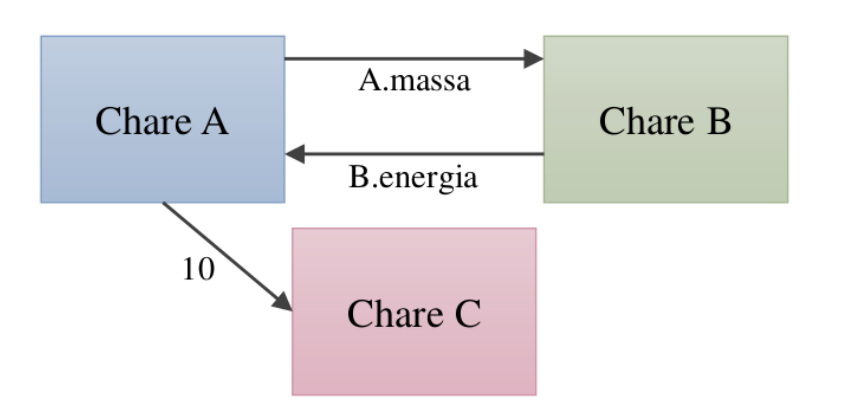
\includegraphics[scale=0.30]{figuras/chares.png}
	\label{img-chare}
    \centering
	\\ Fonte: \cite[p.27]{pilla2015programaccao2}
\end{figure}

Todo programa deve incluir um chare principal que deve ter um ponto de entrada chamado CharmInit. A execução do programa começa pela criação de uma instância do chare principal e a execução de seu ponto de entrada CharmInit ~\cite[p.3]{kale1993parallel2}.

\subsection{Trocas de mensagens}
A troca de mensagens em CHARM++ é feita de forma assíncrona. A troca de mensagens assíncrona faz com que a invocação de um método de entrada em outro chare tenha retorno imediato. Em outras palavras, o chare que envia uma mensagem continu sua execução sem esperar por uma resposta. Adicionalmente, o chare cujo método é chamado pode não começar a executá-lo imediatamente. Esse mecanismo é usado para
guiar a execução da aplicação~\cite[p.28]{pilla2015programaccao2}.

Uma mensagem é uma estrutura constituída por vários campos de dados e é definida de forma semelhante à estrutura de definição em C. As mensagens chegadas são programadas de acordo com uma estratégia de agendamento. A estratégia de agendamento e a estratégia dinâmica de balanceamento de carga são componentes separáveis de modo modular do sistema Charm Runtime, chamado Chare Kernel. O sistema fornece FIFO, LIFO e estratégias de agendamento baseadas em prioridade, com níveis ilimitados de prioridades. Da mesma forma, fornece uma variedade de estratégias dinâmicas de balanceamento de carga desenvolvidas ao longo dos anos. ~\cite{kale1993parallel2}.

Todas as mensagens enviadas para chares em uma unidade de processamento são colocadas em sua fila de mensagens. Cada entrada na fila de mensagens inclui informações sobre qual chare é o receptor, o método invocado e os dados enviados na mensagem ~\cite[p.32]{pilla2015programaccao2}. Como podemos ver na Figura \ref{img-message}. 

\begin{figure}[!htb]
	\centering
	\caption{Distribuição de chares em unidades de processamento e suas filas de mensagens.}
	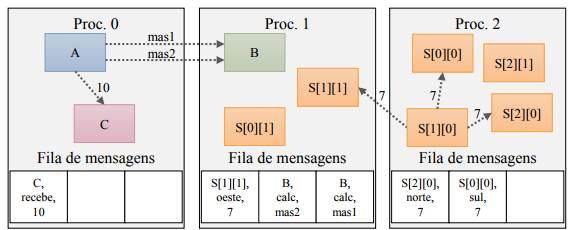
\includegraphics[scale=0.80]{figuras/message.png}
	\label{img-message}
	Fonte: \cite[p.32]{pilla2015programaccao2}
\end{figure}
 
 
 De acordo com ~\cite[p.30]{pilla2015programaccao2} O uso de um modelo de comunicação assíncrona é benéfico pois remove a obrigação de uma sincronização entre o emissor e o receptor de uma mensagem. Isso remove tanto a espera do emissor por uma resposta escondendo parte da latência de comunicação da plataforma quanto o bloqueio da unidade de processamento do receptor enquanto espera pela recepção de uma mensagem.
 
 \subsection{Modelo de execução}
 O processamento nas aplicações em Charm++ é decomposto em objetos chamados chares. O programador implementa as computações e comunicações descrevendo como esses objetos vao interagir e o ambiente de Charm++ gerencia as mensagens geradas por essas interações. Os objetos se comunicam através de chamadas remotas de métodos. Ainda, o ambiente é responsável pelo gerenciamento dos recursos arquiteturais ~\cite{pillaNatalRN}. Na Figura \ref{img-abstracao} podemos ver uma idéa de abstração de aplicação.
 
 \begin{figure}[!htb]
 	\centering
	\caption{Abstração de aplicação na plataforma Charm++}
 	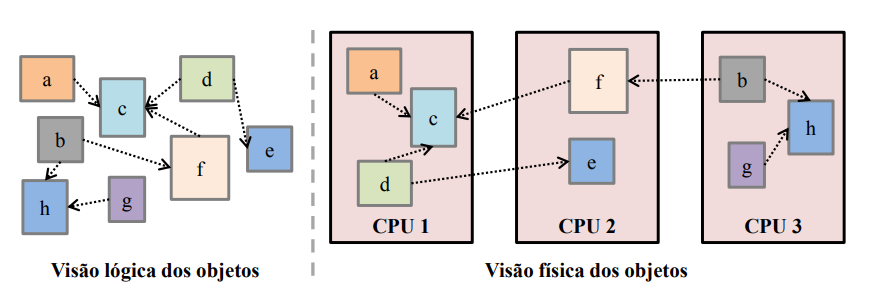
\includegraphics[scale=0.50]{figuras/abstracao.png}
	Fonte: \cite{pillaNatalRN}
 	\label{img-abstracao}
 \end{figure}
 
 No CHARM++, os usuários definem suas aplicações em termos de objetos C++ especiais chamados de chares e coleções indexadas de chares chamados de arrays de chare. Para a maioria, os conjuntos de chares e chare são definidos exatamente como classes padrão e arrays C++, permitindo que o programador aproveite o encapsulamento e abstração de dados. Normalmente, há muitos mais chares do que PEs(processing elements), permitindo que o RTS(Runtime System) aproveite a composição. Como o CHARM ++ usa um paradigma baseado em objetos, o programador também pode implementar facilmente diferentes tipos de unidades de trabalho ~\cite{acun2014parallel}.
 
 No momento em que um projeto do Charm++ é compilado além dos arquivos de cabeçalho com extensão .h e os códigos padrões com extensões .C por exemplo,  o compilador do Charm++ denominado CHARMC utiliza um tradutor que faz a leitura do arquivo de interface. Após a leitura do arquivo de interface são gerados 2 arquivos com extensões .def.h e .decl.h. Após essa etapa o compilador é utilizado novamente para gerar o arquivo de saída com extensão .o. Para rodar a aplicação é necessário utilizar um arquivo de execução do próprio Charm denominado CHARMRUN. Este Fluxo pode ser visto na Figura \ref{img-compiler} a seguir:
 
 \begin{figure}[!htb]
	\centering
	\caption{Processo de compilação de um projeto utilizando CHARM++}
	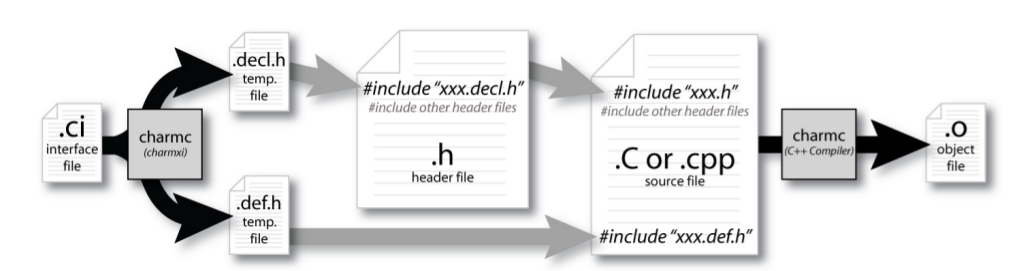
\includegraphics[scale=0.40]{figuras/compile.png}
	\\ Fonte: \cite{compileIMG}
	\label{img-compiler}
\end{figure}

\subsection{Balanceamento de carga}

Muitas estratégias de balanceamento de carga em CHARM++ são baseadas em uma heurística conhecida como princípio da persistência. Ele postula que, empiricamente, para certas classes de aplicações científicas e de engenharia, quando elas são expressadas em um termo de objetos naturais, as cargas computacionais e padrões de comunicação tende a persistir ao longo do tempo, mesmo em cálculos com evolução dinâmica~\cite{zheng2010hierarchical}.
%Many load balancing strategies in CHARM++ are based on a heuristic known as the principle of persistence. It posits that, empirically, for certain classes of scientific and engineering applications, when they are expressed in terms of natural objects (as CHARM++ objects or threads), the computational loads and communication patterns tend to persist over time, eve in dynamically evolving computations. This has led to the development of measurement-based load balancing strategies that use the recent past as a guideline for the near future

De acordo com \cite{pilla2015programaccao2}, O balanceamento de carga em CHARM++ é baseado na medição do tempo de atividade dos chares e das unidades de processamento. Durante um certo período de execução de uma aplicação, o sistema coleta uma serie de informações , esses dados são organizados pelo ambiente em um vetor de informações sobre chares e um vetor de informações sobre unidades de processamento, os quais são encaminhados a um algoritmo de balanceamento de carga. O algoritmo é responsável por avaliar as informações atuais recebidas e prover um novo mapeamento de chares para unidades de processamento. Para habilitar o balanceamento de carga em uma aplicação em CHARM++, o programador é responsável apenas por implementar métodos de serialização para os objetos, por inserir uma chamada ao método bloqueante AtSync() em algum momento da execução de todos os chares e por definir um método de entrada ResumeFromSync(), o qual será chamado após o término do balanceamento de carga. Quando todos os chares alçarem a chamada AtSync, um algoritmo de balanceamento de carga externo, o qual foi compilado em anexo à aplicação e escolhido no momento de sua execução, computará um novo mapeamento.

%Depending on the needs of applications, the user can invoke appropriate load balancer. The load balancing framework in CHARM++ instruments each chare as well as records the PE’s load. In the AtSync mode of load balancing, all the chares pause their execution and call AtSync. The load statistics are collected and the user specified load balancing strategy is used to compute the new mapping. Once the load balancing decision is made, the framework handles the migration of the chares to the newly mapped PEs and resumes them.

 

\section{Considerações do Capítulo}
Neste capítulo foi apresentado os conceitos e definições das diferentes tecnologias relacionadas à computação de alto desempenho. Foi explanado as arquiteturas e plataformas que se encaixam neste contexto, além de apresentar alguns estudos e trabalhos relacionados.

No Capítulo 3, será apresentado o ambiente de trabalho onde os testes foram realizados, especificando as configurações dos dispositivos de processamento, armazenamento e benchmark que foram utilizados para a implementação dos testes.

\chapter{SmartLB}

\section{Proposta}
A grande motivação para o desenvolvimento deste balanceador de carga proveio do desígnio da melhoria e correção de alguns problemas de um BC que utilizando uma abordagem gulosa na composição de seu algoritmo, onde trabalhava com a idéia de calcular a média aritmética do processador e com base nesse calculo então decidir qual tarefa iria ser migrada de fato. O Almejo de um ganho maior de desempenho na realização de testes com grandes cargas computacionais, dimanou na criação de um novo balanceador de carga que também utiliza uma abordagam centralizada, com uma estratégia de tomada de decisão um pouco diferente. Culminando em um ganho significativo de desempenho em relação a este BC específico e também a outros balanceadores que utilizam diferentes estratégias de tomada de decisão. O balanceador de carga em questão levou o nome de \newlb.    

%O BC proposto foi desenvolvido utilizando oframeworkde balanceamento de cargas disponibilizado pelo Charm++. Possui uma abordagem centralizada, o que significa que a estrutura de cargas e de comunicação da maquina, alem de um processo de tomada de decisao, ficam armazenadas em um unico ponto. A escolha de uma abordagem centralizada se deu pelo fato desta realizar um balanceamento mais preciso em relac ̧ao ̃as outras`abordagens. Apesar de trabalhar muito bem com alguns milhares de processadores, podeenfrentar problemas de escalabilidade principalmente em maquinas paralelas com pouca ́memoria.

\section{Metodologias de Implementação}

Atualmente muitas aplicações são dinâmicas ou realizam grandes cálculos computacionais, demandando cada vez de mais capacidade computacional. De acordo com \cite{padoin2014saving}, o grande problema por trás disso é que na maioria das vezes não há uma preocupação com o desbalanceamento de carga gerado por estas aplicações, impedindo que as máquinas paralelas aproveitem todo o seu potencial. Na figura \ref{img_load_balance_unbalance} podemos notar a diferença entre um processador balanceado e um que não está balanceado.

\begin{figure}[!htb]
	\centering
	\caption{Diferença Entre um Processador com Carga Desbalanceada e Balanceada}
	\centering
	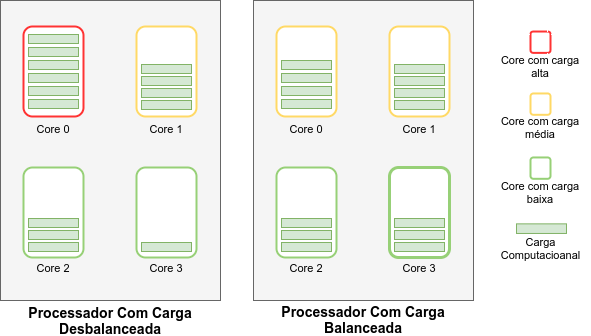
\includegraphics[scale=0.50]{figuras/load_balance.png}
	\label{img_load_balance_unbalance}
	\centering
\end{figure}

Também baseado nesse problema é que o \newlb foi desenvolvido buscando atingir o estado de equilíbrio entre os processadores rapidamente, sem partir diretamente para os chares mais carregados evitando migrações desnecessárias. O BC proposto possui uma abordagem centralizada, então o processo de tomada de decisão e a estrutura de cargas e comunicação da máquina ficam armazenadas em um único computador. Em virtude de realizar um balanceamento de carga mais preciso e trabalhar muito bem com escalabilidade é que foi escolhido a abordagem centralizada.

Durante o processo de execução, o BC coleta dados dos processadores e da aplicação
e os armazena em um banco de dados de balanceamento de cargas. Dentre estas informações,
destacam-se o número total de objetos, a carga total de cada processador, a carga de cada
objeto e o número total de processadores.Estes dados serão utilizados na hora de decidir quais chares devem ser migrados e qual valor cada processador deve ter para estar em equilíbrio.

O \newlb foi desenvolvido utilizando o framework de balanceamento de cargas disponibilizado pelo \charm. Este framework de balanceamento de carga foi escolhido uma vez que permite tanto a criação de um novo BC quanto a utilização dos BCs disponibilizados pelo ambiente para comparações de resultados.

O \charm adota uma metodologia baseada na medição das cargas das tarefas que executam em cada core. Para isso, o framework coleta automaticamente estatísticas da carga computacional e da comunicação destes objetos e armazena tais informações em uma base de dados que pode ser utilizada pelos BC para a tomada de decisões \cite{jyothi2004debugging}.


\section{Algoritmo}

A estratégia utilizada para implementação do balanceamento de carga proposto constitui-se de melhorias nas estrategias utilizadas nos algoritmos \greedylb e \refinelb. Nossas melhorias buscam equilibrar as cargas entre os processadores reduzindo o número de migrações, adotando um threshold para definir o desbalanceamento de carga aceitável.

Na Figura \ref{img_smartlb_effect} é exemplificado o funcionamento da estratégia de tomada de decisão do \newlb. A partir de informações fornecidas pelo \charm, o algoritmo proposto busca atingir ba lanceamento levando em consideração a diferença de carga entre o core mais carregado e o
menos carregado. Desta forma, migra tarefas do core mais carregado para o core com menor carga, buscando equilibrar a carga total do sistema, reduzir o número de migrações e reduzir o tempo total de execução da aplicação.

\begin{figure}[!htb]
	\centering
	\caption{Balanceamento de carga executado pelo \newlb}
	\centering
	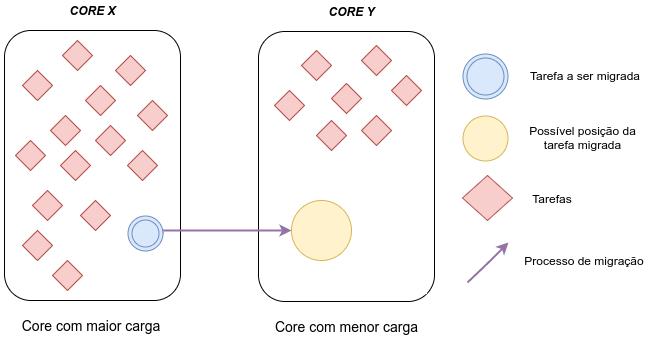
\includegraphics[scale=0.40]{figuras/smartlb_load_balance.png}
	\label{img_smartlb_effect}
	\centering
\end{figure}

Na Tabela 1 são apresentados os principais parâmetros utilizados na implementação do
algoritmo proposto.

\begin{table}[h]
	\centering
	\caption{Principais parâmetros utilizados no algoritmo \newlb}
	\vspace{0.5cm}
	\resizebox{.6\columnwidth}{!}{
		\label{tab:parametros}
		\begin{tabular}{l|l}
			\hline
			\textbf{Parâmetro} & \textbf{Definição} \\
			\hline
			$ PM $ & Processador com maior carga \\
			$ Pm $ & Processador com menor carga \\ 
			
			$ D $ & Desbalanceamento entre $PM$ e $Pm$ \\
			
			$ ct $ & Carga da tarefa $P$ \\
			$ nTarefas $ &  Número de tarefas\\
			
			$ getProcessadorAtual(i) $ & Retorna o processador atual da tarefa\\
			$ getCargaTarefa()     $ & Retorna a carga da tarefa\\
			$ getCargaMaior() 	     $ & Retorna a carga do processador mais carregado \\
			$ getCargaMenor()        $ & Retorna a carga do processador menos carregado \\
			
			$ migrarProcesso(i, PM, Pm) $ & Migrar tarefa $i$ de $ PM $ para $ Pm $ \\
			
			
			\hline
		\end{tabular}
} \end{table}

\begin{table}[h]
	\centering
	%\caption{Algoritmo: \avg}
	%\vspace{0.5cm}
	\resizebox{.4\columnwidth}{!}{
		\label{tab:algoritmo}
		\begin{tabular}{cl}
			%  \hline
			\multicolumn{2}{c}{Algoritmo 1: Implementação do \newlb} \\
			\hline
			& $~~~$\\
			
			1 & $PM = getCargaMaior();$  \\
			2 & $Pm = getCargaMenor();$  \\
			3 & $\textbf{if}( (Pm / PM ) > Threshold)$ \{ \\
			4 & $~~~~~~~\textbf{for}(i=1; i<=nTarefas; i++)$ \{ \\
			5 & $~~~~~~~~~~~~\textbf{if}(getProcessadorAtual(i) == PM)$ \{ \\
			6 & $~~~~~~~~~~~~~~~~ ct = getCargaTarefa(i);$  \\
			7 & $~~~~~~~~~~~~~~~~ D = PM-Pm;$  \\
			8 & $~~~~~~~~~~~~~~~~~ \textbf{if}(ct <= D)$ \{\\
			9 & $~~~~~~~~~~~~~~~~~~~~~~migrarProcesso(i, PM, Pm);$ \\
			10 & $~~~~~~~~~~~~~~~~~~~~~\textbf~ PM = getCargaMaior(); $\\
			11 & $~~~~~~~~~~~~~~~~~~~~~\textbf~ Pm = getCargaMenor(); $\\
			12 & $~~~~~~~~~~~~~~~~~ \}$ \\
			13 & $~~~~~~~~~~~~ \}$ \\
			14 & $~~~~~~ \}$ \\
			15 & $\} $\\
			%     \hline
		\end{tabular}
	}
\end{table} 

Assim, quando o balanceador é aplicado, ele primeiro analisa a diferença de carga entre o processador mais e menos carregado. Caso essa diferença for maior que o \textit{threshold} o balanceador busca tarefas do processador mais carregado testando se a carga da tarefa é menor ou igual ao desbalanceamento. Caso seja, ele realiza a migração desta tarefa do processador mais carregado para o menos carregado e encontra o novo processador mais carregado e o novo processador menos carregado, como demonstrado no Algoritmo 1. 

Desta forma, consegue-se um balanceamento de carga mais preciso, evitando migrações desnecessárias. Após a execução, quando não existem mais processadores a serem mapeados e as cargas de todas as unidades de processamento possuem um valor próximo um do outro, o balanceamento é encerrado. 

\chapter{Metodologia}

\section{Benchmarks}
\section{Hardware Utilizado}
\section{Benchmarks}
Para gerar os resultados os balanceadores de carga foram submetidos a simulações utilizando 3 benchmarks, disponibilizados pelo próprio ambiente de programação \charm. Os benchmarks escolhidos foram o LB\_test, KNeighbor e o Stencil3D, que foram configurados da seguinte forma:
\begin{itemize}
	\item \textbf{LB\_Test}: O benchmark está configurado para realizar 150 iterações por tarefa, com sincronização a cada 10 iterações e uma carga computacional variante entre 1000ms e 150000ms.
	
	\item \textbf{KNeighbor}: O benchmark foi configurado com para realizar testes com 15000 mensagens, 150 iterações por tarefa sendo que o benchmark será sincronizado a cada 10 iterações.
	
	\item \textbf{Stencil3D}: O benchmark foi configurado para executar com 20 blocos, realizando 150 iterações por tarefas com sincronização do benchmark a cada 10 iterações.
\end{itemize} 

Em ambos os benchmarks foram realizados testes alternando entre 50, 100 e 200 tarefas.


\section{Considerações do Capítulo}


\chapter{Resultados  \label{cap:resultados}}

\section{Considerações do Capítulo}

\chapter{Conclusão  \label{cap:conclusão}}

\section{Trabalhos Futuros}


\postextual
% ----------------------------------------------------------
% Referências bibliográficas
% ----------------------------------------------------------
\bibliography{bibliografia}

% ----------------------------------------------------------
% Anexos
% ----------------------------------------------------------

% ---
% Inicia os anexos
% ---

%\input{texto/anexo.tex}


%---------------------------------------------------------------------
% INDICE REMISSIVO
%---------------------------------------------------------------------

%\phantompart
%\printindex

\end{document}